% Options for packages loaded elsewhere
\PassOptionsToPackage{unicode}{hyperref}
\PassOptionsToPackage{hyphens}{url}
%
\documentclass[
  12 pt,
  a4paper,
]{article}
\usepackage{amsmath,amssymb}
\usepackage{setspace}
\usepackage{iftex}
\ifPDFTeX
  \usepackage[T1]{fontenc}
  \usepackage[utf8]{inputenc}
  \usepackage{textcomp} % provide euro and other symbols
\else % if luatex or xetex
  \usepackage{unicode-math} % this also loads fontspec
  \defaultfontfeatures{Scale=MatchLowercase}
  \defaultfontfeatures[\rmfamily]{Ligatures=TeX,Scale=1}
\fi
\usepackage{lmodern}
\ifPDFTeX\else
  % xetex/luatex font selection
  \setmainfont[]{Times New Roman}
\fi
% Use upquote if available, for straight quotes in verbatim environments
\IfFileExists{upquote.sty}{\usepackage{upquote}}{}
\IfFileExists{microtype.sty}{% use microtype if available
  \usepackage[]{microtype}
  \UseMicrotypeSet[protrusion]{basicmath} % disable protrusion for tt fonts
}{}
\makeatletter
\@ifundefined{KOMAClassName}{% if non-KOMA class
  \IfFileExists{parskip.sty}{%
    \usepackage{parskip}
  }{% else
    \setlength{\parindent}{0pt}
    \setlength{\parskip}{6pt plus 2pt minus 1pt}}
}{% if KOMA class
  \KOMAoptions{parskip=half}}
\makeatother
\usepackage{xcolor}
\usepackage[margin=1in]{geometry}
\usepackage{color}
\usepackage{fancyvrb}
\newcommand{\VerbBar}{|}
\newcommand{\VERB}{\Verb[commandchars=\\\{\}]}
\DefineVerbatimEnvironment{Highlighting}{Verbatim}{commandchars=\\\{\}}
% Add ',fontsize=\small' for more characters per line
\usepackage{framed}
\definecolor{shadecolor}{RGB}{248,248,248}
\newenvironment{Shaded}{\begin{snugshade}}{\end{snugshade}}
\newcommand{\AlertTok}[1]{\textcolor[rgb]{0.94,0.16,0.16}{#1}}
\newcommand{\AnnotationTok}[1]{\textcolor[rgb]{0.56,0.35,0.01}{\textbf{\textit{#1}}}}
\newcommand{\AttributeTok}[1]{\textcolor[rgb]{0.13,0.29,0.53}{#1}}
\newcommand{\BaseNTok}[1]{\textcolor[rgb]{0.00,0.00,0.81}{#1}}
\newcommand{\BuiltInTok}[1]{#1}
\newcommand{\CharTok}[1]{\textcolor[rgb]{0.31,0.60,0.02}{#1}}
\newcommand{\CommentTok}[1]{\textcolor[rgb]{0.56,0.35,0.01}{\textit{#1}}}
\newcommand{\CommentVarTok}[1]{\textcolor[rgb]{0.56,0.35,0.01}{\textbf{\textit{#1}}}}
\newcommand{\ConstantTok}[1]{\textcolor[rgb]{0.56,0.35,0.01}{#1}}
\newcommand{\ControlFlowTok}[1]{\textcolor[rgb]{0.13,0.29,0.53}{\textbf{#1}}}
\newcommand{\DataTypeTok}[1]{\textcolor[rgb]{0.13,0.29,0.53}{#1}}
\newcommand{\DecValTok}[1]{\textcolor[rgb]{0.00,0.00,0.81}{#1}}
\newcommand{\DocumentationTok}[1]{\textcolor[rgb]{0.56,0.35,0.01}{\textbf{\textit{#1}}}}
\newcommand{\ErrorTok}[1]{\textcolor[rgb]{0.64,0.00,0.00}{\textbf{#1}}}
\newcommand{\ExtensionTok}[1]{#1}
\newcommand{\FloatTok}[1]{\textcolor[rgb]{0.00,0.00,0.81}{#1}}
\newcommand{\FunctionTok}[1]{\textcolor[rgb]{0.13,0.29,0.53}{\textbf{#1}}}
\newcommand{\ImportTok}[1]{#1}
\newcommand{\InformationTok}[1]{\textcolor[rgb]{0.56,0.35,0.01}{\textbf{\textit{#1}}}}
\newcommand{\KeywordTok}[1]{\textcolor[rgb]{0.13,0.29,0.53}{\textbf{#1}}}
\newcommand{\NormalTok}[1]{#1}
\newcommand{\OperatorTok}[1]{\textcolor[rgb]{0.81,0.36,0.00}{\textbf{#1}}}
\newcommand{\OtherTok}[1]{\textcolor[rgb]{0.56,0.35,0.01}{#1}}
\newcommand{\PreprocessorTok}[1]{\textcolor[rgb]{0.56,0.35,0.01}{\textit{#1}}}
\newcommand{\RegionMarkerTok}[1]{#1}
\newcommand{\SpecialCharTok}[1]{\textcolor[rgb]{0.81,0.36,0.00}{\textbf{#1}}}
\newcommand{\SpecialStringTok}[1]{\textcolor[rgb]{0.31,0.60,0.02}{#1}}
\newcommand{\StringTok}[1]{\textcolor[rgb]{0.31,0.60,0.02}{#1}}
\newcommand{\VariableTok}[1]{\textcolor[rgb]{0.00,0.00,0.00}{#1}}
\newcommand{\VerbatimStringTok}[1]{\textcolor[rgb]{0.31,0.60,0.02}{#1}}
\newcommand{\WarningTok}[1]{\textcolor[rgb]{0.56,0.35,0.01}{\textbf{\textit{#1}}}}
\usepackage{longtable,booktabs,array}
\usepackage{calc} % for calculating minipage widths
% Correct order of tables after \paragraph or \subparagraph
\usepackage{etoolbox}
\makeatletter
\patchcmd\longtable{\par}{\if@noskipsec\mbox{}\fi\par}{}{}
\makeatother
% Allow footnotes in longtable head/foot
\IfFileExists{footnotehyper.sty}{\usepackage{footnotehyper}}{\usepackage{footnote}}
\makesavenoteenv{longtable}
\usepackage{graphicx}
\makeatletter
\def\maxwidth{\ifdim\Gin@nat@width>\linewidth\linewidth\else\Gin@nat@width\fi}
\def\maxheight{\ifdim\Gin@nat@height>\textheight\textheight\else\Gin@nat@height\fi}
\makeatother
% Scale images if necessary, so that they will not overflow the page
% margins by default, and it is still possible to overwrite the defaults
% using explicit options in \includegraphics[width, height, ...]{}
\setkeys{Gin}{width=\maxwidth,height=\maxheight,keepaspectratio}
% Set default figure placement to htbp
\makeatletter
\def\fps@figure{htbp}
\makeatother
\setlength{\emergencystretch}{3em} % prevent overfull lines
\providecommand{\tightlist}{%
  \setlength{\itemsep}{0pt}\setlength{\parskip}{0pt}}
\setcounter{secnumdepth}{-\maxdimen} % remove section numbering
\ifLuaTeX
\usepackage[bidi=basic]{babel}
\else
\usepackage[bidi=default]{babel}
\fi
\babelprovide[main,import]{spanish}
\ifPDFTeX
\else
\babelfont{rm}[]{Times New Roman}
\fi
% get rid of language-specific shorthands (see #6817):
\let\LanguageShortHands\languageshorthands
\def\languageshorthands#1{}
\ifLuaTeX
  \usepackage{selnolig}  % disable illegal ligatures
\fi
\usepackage{bookmark}
\IfFileExists{xurl.sty}{\usepackage{xurl}}{} % add URL line breaks if available
\urlstyle{same}
\hypersetup{
  pdfauthor={Tomàs Ferrandis Moscardó},
  pdflang={es-ES},
  hidelinks,
  pdfcreator={LaTeX via pandoc}}

\title{U7-OpenLDAP}
\usepackage{etoolbox}
\makeatletter
\providecommand{\subtitle}[1]{% add subtitle to \maketitle
  \apptocmd{\@title}{\par {\large #1 \par}}{}{}
}
\makeatother
\subtitle{Introducció i instal·lació}
\author{Tomàs Ferrandis Moscardó}
\date{}

\begin{document}
\maketitle

{
\setcounter{tocdepth}{2}
\tableofcontents
}
\setstretch{1.5}
\section{1. SERVICI DE DIRECTORI}\label{servici-de-directori}

Recrodem que un servici de directori és una base de dades jeràrquica i
centralitzada que s'utilitza per emmagatzemar i gestionar informació
clau d'una organització. Aquesta informació pot incloure:

\begin{itemize}
\tightlist
\item
  Gestió d'usuaris i grups.
\item
  Autenticació d'usuaris.
\item
  Drets d'ús en la xarxa i les màquines.
\item
  Configuracions relacionades amb sistemes i aplicacions.
\item
  Autorització i assignació de permisos sobre el sistema de fitxers.
\item
  Gestió centralitzada de recursos de la xarxa com impressores o equips.
\end{itemize}

\section{2. LDAP}\label{ldap}

LDAP (Lightweight Directory Access Protocol) és un protocol estàndard i
multiplataforma per accedir i gestionar serveis de directori. Entre les
característiques principals de LDAP, destaquen:

\begin{itemize}
\tightlist
\item
  La seua independència del sistema operatiu.
\item
  La capacitat de gestionar informació jeràrquica.
\item
  La possibilitat d'autenticació centralitzada en grans xarxes.
\end{itemize}

Usos principals: - Autenticació d'usuaris. - Cerca i recuperació
d'informació en bases de dades jeràrquiques.

\textbf{LDAP no està lligat a cap sistema operatiu} específic i és
compatible amb diferents implementacions de serveis de directori com
OpenLDAP, Active Directory, Novell eDirectory o Oracle Directory Server.

\section{3. OpenLDAP}\label{openldap}

OpenLDAP és una implementació de codi obert del protocol LDAP. Es tracta
d'una solució molt utilitzada en \textbf{entorns Linux} per implementar
serveis de directori lleugers i altament configurables.

En un sistema Linux, OpenLDAP és sovint utilitzat com a nucli per
proporcionar autenticació centralitzada i gestionar l'accés a recursos
de la xarxa. Tot i això, no inclou funcions integrades com DNS o
Kerberos, per la qual cosa sol integrar-se amb altres components per
ampliar la funcionalitat.

Característiques destacades d'OpenLDAP:

\begin{itemize}
\tightlist
\item
  És una solució lleugera i modular.
\item
  Suporta personalització avançada dels esquemes de dades.
\item
  És altament compatible amb altres aplicacions i serveis que
  implementen LDAP.
\end{itemize}

A més, com hem dit, OpenLDAP pot integrar-se amb altres serveis com
Kerberos o Samba per a ampliar les seues funcionalitats.

\section{4. OpenLDAP vs ACTIVE
DIRECTORY}\label{openldap-vs-active-directory}

\subsection{Similituds}\label{similituds}

\begin{enumerate}
\def\labelenumi{\arabic{enumi}.}
\tightlist
\item
  \textbf{Basats en el protocol LDAP:} Tant OpenLDAP com Active
  Directory utilitzen el protocol LDAP com a base per gestionar i
  accedir a la informació.
\item
  \textbf{Directori jeràrquic:} Tots dos estructuren la informació en
  forma d'arbre, amb nodes com dominis, unitats organitzatives (OUs),
  usuaris i grups.
\item
  \textbf{Autenticació centralitzada:} Ambdues solucions permeten
  autenticar usuaris i gestionar recursos de manera centralitzada en una
  xarxa.
\item
  \textbf{Multiplataforma:} Encara que Active Directory està més
  orientat a Windows, amb configuracions addicionals també pot treballar
  amb clients Linux, mentre que OpenLDAP és compatible amb diverses
  plataformes.
\end{enumerate}

\subsection{Diferències}\label{diferuxe8ncies}

\begin{enumerate}
\def\labelenumi{\arabic{enumi}.}
\tightlist
\item
  \textbf{Funcionalitats integrades:}

  \begin{itemize}
  \tightlist
  \item
    Active Directory és un servei complet que inclou LDAP, Kerberos i
    DNS integrats, a més de funcions avançades com Group Policies
    (GPOs).
  \item
    OpenLDAP és una implementació lleugera del protocol LDAP que
    requereix integracions externes per proporcionar funcionalitats
    similars.
  \end{itemize}
\item
  \textbf{Entorn:}

  \begin{itemize}
  \tightlist
  \item
    Active Directory està optimitzat per a xarxes Windows.
  \item
    OpenLDAP és més flexible i està dissenyat principalment per entorns
    Linux/Unix.
  \end{itemize}
\item
  \textbf{Gestió:}

  \begin{itemize}
  \tightlist
  \item
    Active Directory ofereix eines gràfiques com l'Active Directory
    Users and Computers (ADUC) que simplifiquen la gestió però també
    cmdLets (POwerShell)
  \item
    OpenLDAP és configurat principalment a través de fitxers de
    configuració i eines de línia d'ordres però també té entorns gràfics
    com JXplorer.
  \end{itemize}
\end{enumerate}

\subsection{Punts de connexió}\label{punts-de-connexiuxf3}

\begin{enumerate}
\def\labelenumi{\arabic{enumi}.}
\tightlist
\item
  \textbf{Integració en entorns híbrids:} OpenLDAP es pot utilitzar com
  a complement o com a directori secundari en xarxes on Active Directory
  és el directori principal.
\item
  \textbf{Autenticació conjunta:} Mitjançant connectors com
  \textbf{Samba} (que estudiarem al curs) o \textbf{SSSD}, els sistemes
  Linux que utilitzen OpenLDAP poden autenticar-se en dominis d'Active
  Directory.
\item
  \textbf{Sincronització:} Es poden configurar sincronitzacions
  bidireccionals entre OpenLDAP i Active Directory per mantenir la
  coherència de dades entre els dos sistemes.
\end{enumerate}

\subsection{Conclusions}\label{conclusions}

OpenLDAP i Active Directory tenen objectius similars en la gestió
centralitzada d'usuaris i recursos, però cada solució està optimitzada
per a entorns diferents:

\begin{itemize}
\tightlist
\item
  \textbf{OpenLDAP:} És ideal per a entorns Linux que necessiten
  flexibilitat i personalització, especialment quan es prefereix una
  arquitectura modular amb components externs com Kerberos i DNS.
\item
  \textbf{Active Directory:} És la solució preferida per a xarxes
  Windows gràcies a les seues funcionalitats integrades i eines
  d'administració simplificades.
\end{itemize}

La integració entre ambdues eines permet aprofitar el millor de cada una
en xarxes híbrides, oferint una gestió centralitzada i eficient en
entorns complexos.

\section{2 ESTRUCTURA DE LA BD/DIRECTORI
LDAP}\label{estructura-de-la-bddirectori-ldap}

\subsection{2.1 Entrades, objectes i
atributs}\label{entrades-objectes-i-atributs}

La base de dades LDAP té una estructura jeràrquica. Bàsicament totes les
dades s'emmagatzemen en alguna part del directori LDAP, i a similitud
dels directoris de fitxers, aquest directori s'organitza en arbre.

El model d'informació de LDAP està basat en entrades. Cada
\textbf{entrada és un objecte del directori} i conté una col·lecció
d'atributs, alguns dels quals son definitoris o identificadors. El DN o
Distinguished Name, per exemple és únic i global (identifica a tot el
domini de forma única l'ojecte).

Fent un símil amb la taula d'una base de dades relacional, \textbf{una
entrada seria com un registre (fila de la taula) i un atribut seria com
un camp (la columna de la taula).}

A partir d'un exemple ho vorem més clar.

\subsection{2.2 Exemple.}\label{exemple.}

L'alumnat de 2 SMXB, després de la visita al Programa Lanzadera ha
decidit muntar una empresa. Al domini li han posa de nom \emph{smx2b}
amb l'extensió \emph{.com}.

Aquí tens una taula amb els atributs i exemples corresponents:

\begin{longtable}[]{@{}
  >{\raggedright\arraybackslash}p{(\columnwidth - 4\tabcolsep) * \real{0.1026}}
  >{\raggedright\arraybackslash}p{(\columnwidth - 4\tabcolsep) * \real{0.5026}}
  >{\raggedright\arraybackslash}p{(\columnwidth - 4\tabcolsep) * \real{0.3949}}@{}}
\toprule\noalign{}
\begin{minipage}[b]{\linewidth}\raggedright
\textbf{Atribut}
\end{minipage} & \begin{minipage}[b]{\linewidth}\raggedright
\textbf{Definició}
\end{minipage} & \begin{minipage}[b]{\linewidth}\raggedright
\textbf{Exemple}
\end{minipage} \\
\midrule\noalign{}
\endhead
\bottomrule\noalign{}
\endlastfoot
\textbf{RDN} & Nom relatiu dins d'una entrada del directori LDAP. &
\texttt{cn=comercials} \texttt{uid=Arantxa} \\
\textbf{DN} & Camí complet i únic que identifica una entrada al
directori. & \texttt{cn=comercials,ou=DelegacioValencia,dc=smx2b,dc=com}
\texttt{uid=Arantxa,ou=DelegacioValencia,dc=smx2b,dc=com} \\
\textbf{\texttt{cn}} & Nom comú que identifica un grup o una persona. &
\texttt{cn=comercials} \texttt{cn=Arantxa} \\
\textbf{\texttt{uid}} & Identificador únic d'un usuari. &
\texttt{uid=Arantxa} \\
\textbf{\texttt{gidNumber}} & Identificador numèric d'un grup al qual
pertany una entrada (especialment en sistemes UNIX). &
\texttt{gidNumber:\ 10001} \\
\textbf{\texttt{objectClass}} & Classes que defineixen el tipus
d'entrada i els atributs que pot tenir. &
\texttt{objectClass:\ posixGroup}, \texttt{objectClass:\ inetOrgPerson},
\texttt{objectClass:\ top} \\
\textbf{\texttt{homeDirectory}} & Ruta del directori personal d'un
usuari (en sistemes UNIX). & \texttt{/home/smx2b/arantxa} \\
\end{longtable}

\subsection{2.3 Atributs (RDN, DN, CN\ldots)}\label{atributs-rdn-dn-cn}

Totes les entrades emmagatzemades en un directori LDAP tenen un únic
\textbf{``Distinguished Name,'' o DN}.

El DN per a cada entrada està compost de dos parts:

\begin{itemize}
\tightlist
\item
  el Nom Relatiu Distingit (\textbf{RDN} per les seves sigles en anglès,
  Relative Distinguished Name)
\item
  la localització dins del directori LDAP on el registre resideix.
\end{itemize}

El RDN és la porció de la teva DN que no està relacionada amb
l'estructura de l'arbre de directori.

La majoria dels objectes que emmagatzemes en un directori LDAP tindrà un
nom, i el nom és emmagatzemat freqüentment en l'atribut cn (Common
Name). Ja que pràcticament tot té un nom, la majoria dels objectes que
emmagatzemarà LDAP utilitzen el seu valor cn com a base per a la seva
RDN.

Exemple:

\begin{Shaded}
\begin{Highlighting}[]
\ExtensionTok{dn:}\NormalTok{ cn=comercials,ou=DelegacioValencia,dc=smx2b,dc=com}
\ExtensionTok{cn:}\NormalTok{ comercials}
\ExtensionTok{gidNumber:}\NormalTok{ 10001}
\ExtensionTok{objectClass:}\NormalTok{ posixGroup}
\ExtensionTok{objectClass:}\NormalTok{ top}
\ExtensionTok{memberUid:}\NormalTok{ 1001}
\end{Highlighting}
\end{Shaded}

• El DN base del meu directori ou = DelegacioNord, dc = smx2b, dc = com
• El RDN d'un registre d'un grup cn=comercials

Per als comptes d'usuari, típicament veuràs un DN basat en el cn o al
uid (ID de l'usuari). Per exemple, el DN del comercial de login: arantxa
pot semblar-se a:

\begin{Shaded}
\begin{Highlighting}[]
\ExtensionTok{dn:}\NormalTok{ uid=Arantxa,ou=DelegacioValencia,dc=smx2b,dc=com}
\ExtensionTok{cn:}\NormalTok{ Arantxa}
\ExtensionTok{gidNumber:}\NormalTok{ 10001}
\ExtensionTok{homeDirectory:}\NormalTok{ /home/smx2b/arantxa}
\ExtensionTok{objectClass:}\NormalTok{ inetOrgPerson}
\ExtensionTok{objectClass:}\NormalTok{ organizationalPerson}
\ExtensionTok{objectClass:}\NormalTok{ posixAccount}
\ExtensionTok{objectClass:}\NormalTok{ person}
\ExtensionTok{objectClass:}\NormalTok{ top}
\end{Highlighting}
\end{Shaded}

LDAP utilitzen uid per a indicar ``ID de l'usuari'', no s'ha de
confondre amb el número uid de UNIX. La majoria de les empreses intenten
donar a cadascun un nom de login, així aquesta aproximació fa que tinga
sentit emmagatzemar informació sobre els empleats.

Pero podem usar el cn també.

Aquí veiem l'entrada Nom Comú o CN (per les seves sigles en anglès,
common name) utilitzada. En el cas d'un registre LDAP per a una persona,
pensa en el nom comú com els seu nom complet. Un pot veure fàcilment
l'efecte col·lateral d'aquesta forma: si el nom canvia, el registre LDAP
ha de ``moure'' d'un DN a un altre.

\section{3 INSTAL·LACIÓ en el
SERVIDOR}\label{installaciuxf3-en-el-servidor}

\subsection{3.1 Preparar el servidor
Ubuntu}\label{preparar-el-servidor-ubuntu}

Nom de la màquina virtual i de l'equip: ubuntuserver1 Usuari principal:
admin Contrasenya usuari principal: Gandia2425

Dos targetes de xarxa (en Virtualització) NAT --\textgreater{} DHCP
Xarxa Interna, interfície inet -\textgreater{} Manual

(al món real la NAT correspondria a una NIC connectada al router amb
eixida a internet i la xarxa interna al switch de la LAN)

\subsubsection{3.1.1 Configurar la targeta de
xarxa}\label{configurar-la-targeta-de-xarxa}

Editem la configuració de la segona targeta de xarxa, la de xarxa
interna, i li fiquem una IP fixa i la màscara. En el meu cas utilitzaré
l'IP 192.168.1.1. Busque el fitxer i l'edite amb nano

\begin{Shaded}
\begin{Highlighting}[]
\FunctionTok{sudo}\NormalTok{ nano /etc/netplan/50{-}cloud{-}init.yaml}
\FunctionTok{sudo}\NormalTok{ netplan apply}
\ExtensionTok{ip}\NormalTok{ a}
\end{Highlighting}
\end{Shaded}

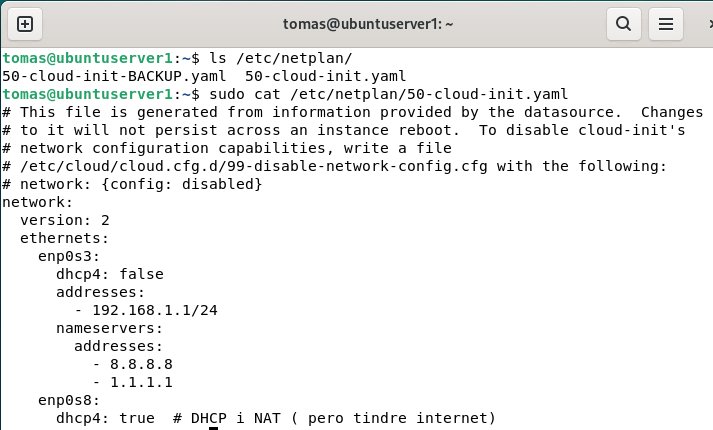
\includegraphics{png/netplan.png}

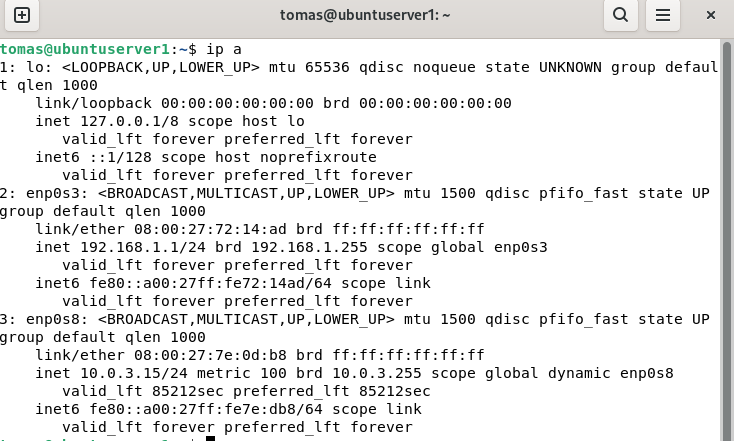
\includegraphics{png/ipa.png}

\subsubsection{3.1.2 Nom de màquina}\label{nom-de-muxe0quina}

\begin{itemize}
\tightlist
\item
  Consultem el nom del servidor
\end{itemize}

\begin{Shaded}
\begin{Highlighting}[]
\FunctionTok{sudo}\NormalTok{ cat /etc/hostname}
\end{Highlighting}
\end{Shaded}

(o echo \$HOSTNAME)

\begin{itemize}
\tightlist
\item
  Modifiquem el fitxer de noms
\end{itemize}

\begin{Shaded}
\begin{Highlighting}[]
\FunctionTok{sudo}\NormalTok{ nano /etc/hosts}
\end{Highlighting}
\end{Shaded}

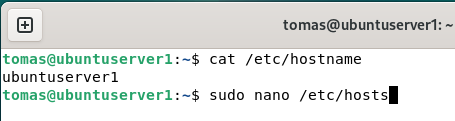
\includegraphics{png/hosts.png}

Afegim la tercera línia:

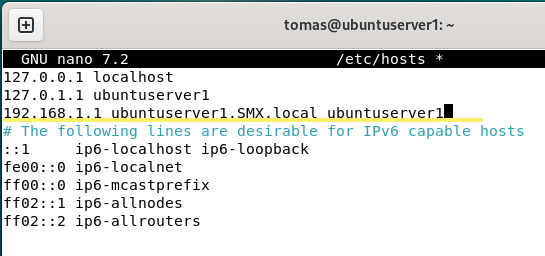
\includegraphics{png/hosts1.png}

Cal reiniciar el servidor

\begin{Shaded}
\begin{Highlighting}[]
\ExtensionTok{reboot}
\end{Highlighting}
\end{Shaded}

\subsection{3.2 Instal·lar el OpenLDAP}\label{installar-el-openldap}

\begin{itemize}
\tightlist
\item
  Actualitzem repositori i software prèviament
\end{itemize}

\begin{Shaded}
\begin{Highlighting}[]
\FunctionTok{sudo}\NormalTok{ apt update }\KeywordTok{\&\&} \FunctionTok{sudo}\NormalTok{ apt upgrade}
\end{Highlighting}
\end{Shaded}

\begin{itemize}
\tightlist
\item
  Instal·lem
\end{itemize}

\begin{Shaded}
\begin{Highlighting}[]
\FunctionTok{sudo}\NormalTok{ apt install slapd ldap{-}utils }\AttributeTok{{-}y}
\end{Highlighting}
\end{Shaded}

Si no s'inicia l'assistent, executa\ldots{}

\begin{Shaded}
\begin{Highlighting}[]
\FunctionTok{sudo}\NormalTok{ dpkg{-}reconfigure slapd}
\end{Highlighting}
\end{Shaded}

• Ens pregunta si volem ometre l'assistent: Seleccionem: no

• Ens pregunta la base del nostre \textbf{domini DNS:} En el meu cas:
\textbf{smx2b.com}

• Ens pregunta el nom complet de l'\textbf{organització:} En el meu cas:
\textbf{smx2b}

• Ens pregunta la paraula de pas. És la que usarem amb \emph{admin} més
avant per connectar-nos.

• A les següents preguntes podeu deixar l'opció per defecte.

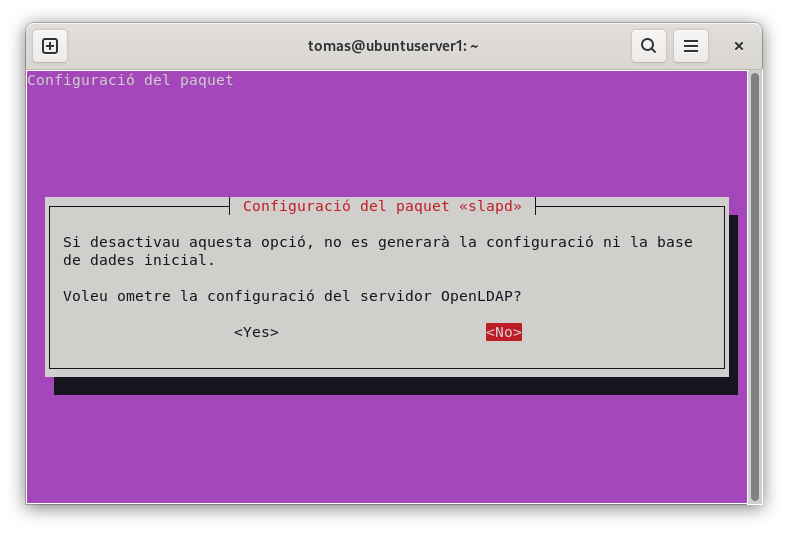
\includegraphics{png/ometreConfiguracio.png}

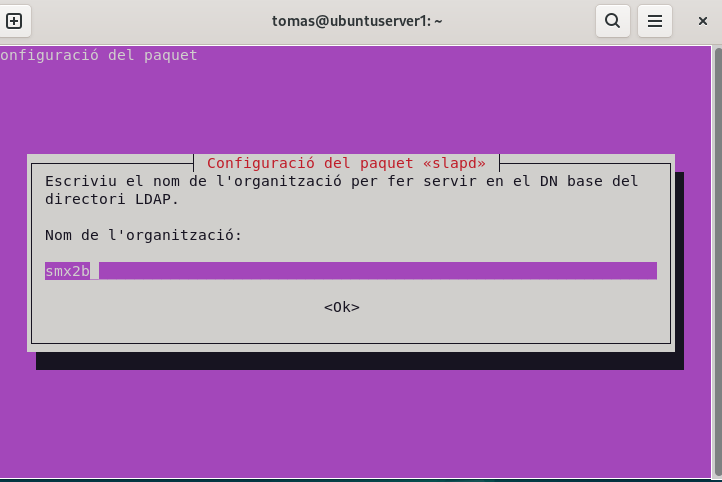
\includegraphics{png/slapd3.png}

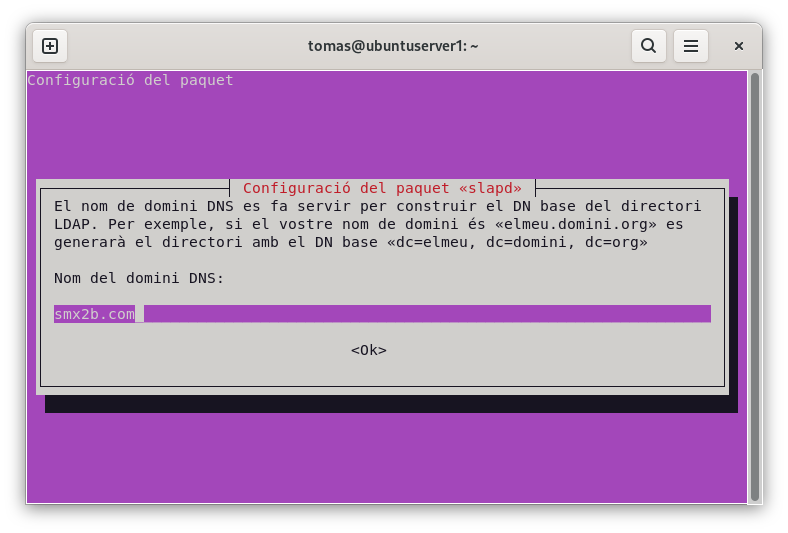
\includegraphics{png/slapdDNS.png}

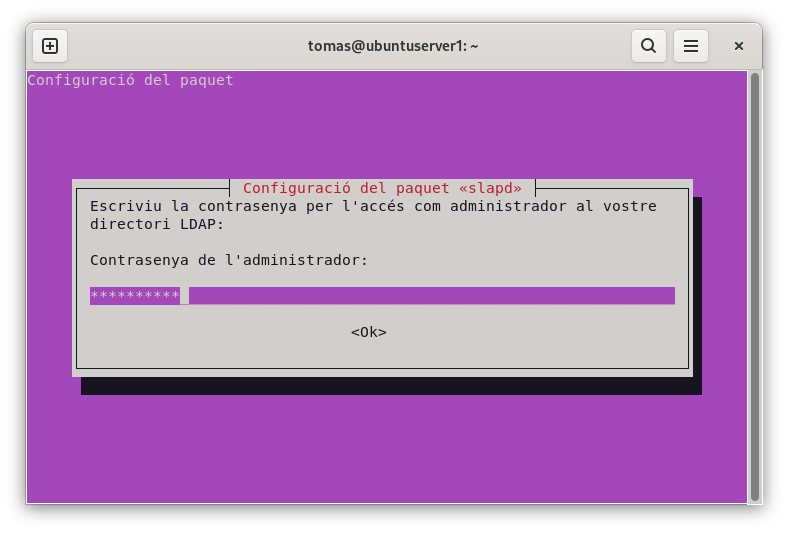
\includegraphics{png/slapdPASSWORD.png}

\subsubsection{Comprovar el resultat}\label{comprovar-el-resultat}

\begin{Shaded}
\begin{Highlighting}[]
\FunctionTok{sudo}\NormalTok{ slapcat}
\end{Highlighting}
\end{Shaded}

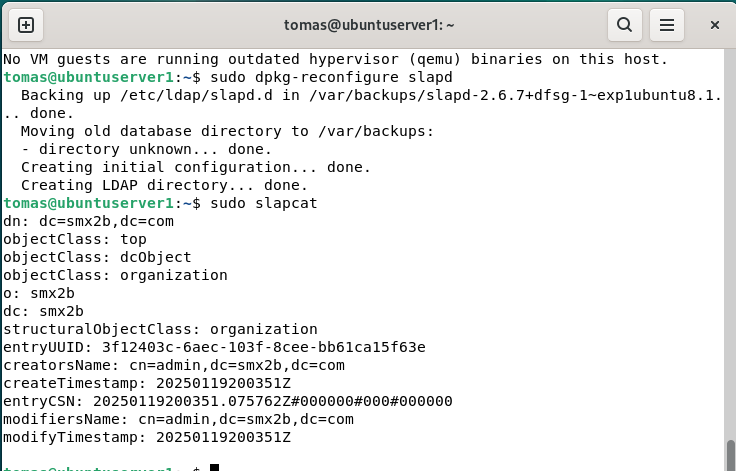
\includegraphics{png/slapd4.png}

\subsubsection{Reiniciar el servici}\label{reiniciar-el-servici}

\begin{Shaded}
\begin{Highlighting}[]
\FunctionTok{sudo}\NormalTok{ systemctl restart slapd}
\end{Highlighting}
\end{Shaded}

Amb \emph{status} podem comprovar si está ``running''.

\section{4. INSTAL·LACIÓ en el CLIENT
UBUNTU}\label{installaciuxf3-en-el-client-ubuntu}

\subsection{4.1 Configuració de la NIC}\label{configuraciuxf3-de-la-nic}

Xarxa interna --\textgreater{} Manual

Podem optar per modificar el netplan com hem fet en el servidor o
gràficament. Alguns Entorns d'Escriptori com el LXQt de Lubuntu ho
failiten prou:

\includegraphics{png/configuracioAvançadadeXarxa2.jpg}

Comprovem la connectivitat entre Servidor i Client

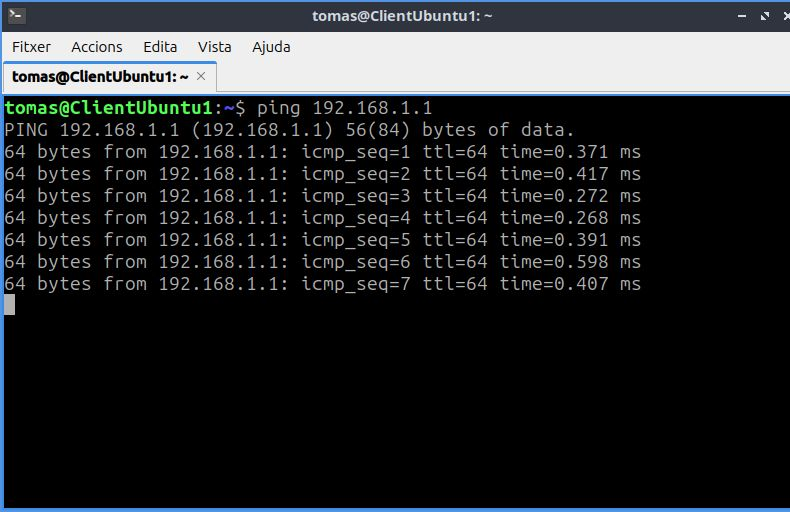
\includegraphics{png/pingIpServidor.jpg}

\subsection{4.2 Configurar la resolució de
noms.}\label{configurar-la-resoluciuxf3-de-noms.}

Associació del nom del servidor a la seua IP en el \textbf{/etc/hosts}

\begin{Shaded}
\begin{Highlighting}[]
\FunctionTok{sudo}\NormalTok{ nano /etc/hosts}
\end{Highlighting}
\end{Shaded}

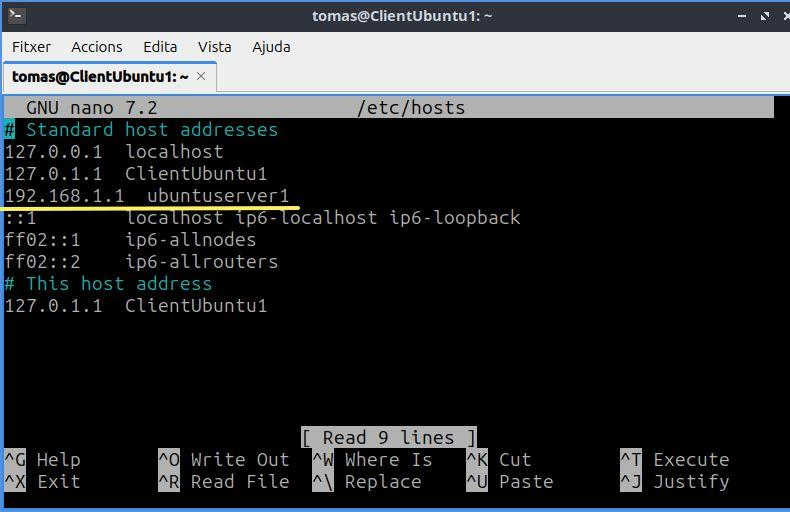
\includegraphics{png/host.jpg}

Comprovem que funciona la resolució de noms

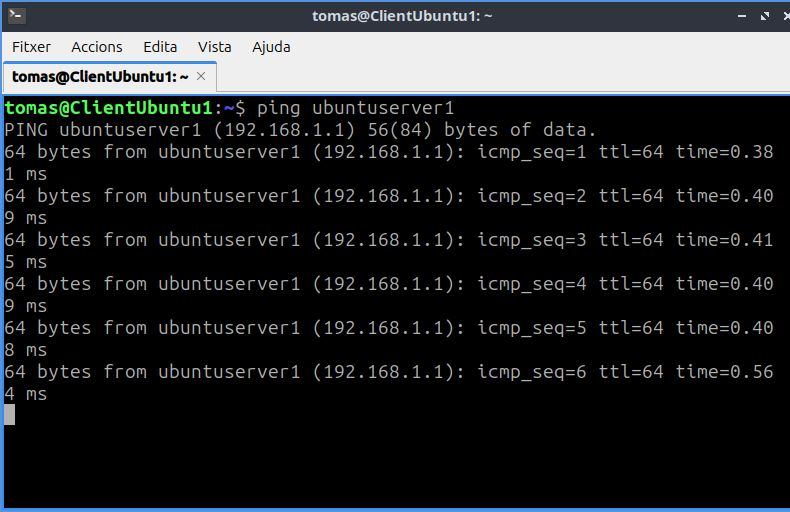
\includegraphics{png/pingNomServidor.jpg}

\section{5 JXPLORER}\label{jxplorer}

Existeixen varies aplicacions gràfiques per a facilitar la gestió
d'LDAP: Jxplorer, phpLDAPadmin i Apache Directory Studio.

Anem a provar el JXPLORER instal·lada en el client. Pot instal·lar-se en
el servidor però la majoria de servidors Linux no tindran entorn gràfic.

\subsection{5.1 Instal·lació del JXplorer en el
client}\label{installaciuxf3-del-jxplorer-en-el-client}

Instal·lem requisists previs

\begin{Shaded}
\begin{Highlighting}[]
\FunctionTok{sudo}\NormalTok{ apt install openjdk{-}11{-}jdk}
\end{Highlighting}
\end{Shaded}

Ara ja si podem instal·lar el programa Jxplorer

\begin{Shaded}
\begin{Highlighting}[]
    \FunctionTok{sudo}\NormalTok{ apt install jxplorer}
\end{Highlighting}
\end{Shaded}

Un vegada l'engeguem des de l'icona, hem de \textbf{connectar amb el
servidor}.

Important: El client executarà jxplorer, però haurà de connectar amb el
servidor ldap.

\begin{itemize}
\item
  Si estiguérem al servidor indicaríem \emph{127.0.0.1 o localhost}. Al
  nostre cas (instal·lació en el client) caldrà indicar la IP del
  servidor.
\item
  Hem de triar l'opció de \textbf{Usuari + Password} que és la que hem
  configurat en instal·lar el sevici i\ldots{}
\item
  indicar el password que també hem introduït en la configuració
\end{itemize}

\section{6 ELS OBJECTES PRINCIPALS}\label{els-objectes-principals}

Anem a crear i modificar Unitats Organitzatives, grups d'usuaris i
usuaris del domini. I amb la creació des del \emph{jXplorer} podrem
introduir uns conceptes bàsics de teoria sobre el LDAP perquè ens cladrà
conéixer les \textbf{propietats mínimes} fan falta en cada objecte.

\subsection{6.1 Propietats: classes i
atributs}\label{propietats-classes-i-atributs}

Les propietats que veiem quan donem d'alta una Unitat Organitzativa, un
usuari o un grup poden ser:

\begin{itemize}
\tightlist
\item
  \textbf{Classes:} Esquemes que defineixen què pot o ha de tenir un
  objecte.\\
\item
  \textbf{Atributs:} Dades concretes d'un objecte definides per les
  classes.
\end{itemize}

\begin{longtable}[]{@{}
  >{\raggedright\arraybackslash}p{(\columnwidth - 4\tabcolsep) * \real{0.2137}}
  >{\raggedright\arraybackslash}p{(\columnwidth - 4\tabcolsep) * \real{0.3846}}
  >{\raggedright\arraybackslash}p{(\columnwidth - 4\tabcolsep) * \real{0.4017}}@{}}
\toprule\noalign{}
\begin{minipage}[b]{\linewidth}\raggedright
\textbf{Característica}
\end{minipage} & \begin{minipage}[b]{\linewidth}\raggedright
\textbf{Classes (objectClass)}
\end{minipage} & \begin{minipage}[b]{\linewidth}\raggedright
\textbf{Atributs}
\end{minipage} \\
\midrule\noalign{}
\endhead
\bottomrule\noalign{}
\endlastfoot
\textbf{Funció} & Defineixen el tipus d'objecte i els seus atributs &
Contenen dades específiques de l'objecte \\
\textbf{Tipus} & Estructural, auxiliar o abstracte & Obligatori
(\texttt{must}) o opcional (\texttt{may}) \\
\textbf{Exemple} & \texttt{inetOrgPerson}, \texttt{posixAccount},
\texttt{top} & \texttt{cn}, \texttt{uid}, \texttt{mail},
\texttt{gidNumber}, \texttt{sn} \\
\textbf{Obligatorietat} & Cada entrada LDAP ha de tenir almenys una
classe & Només els atributs marcats com a \texttt{must} són
obligatoris \\
\textbf{Herència} & Pot heretar atributs d'altres classes & No hereten,
són definits per les classes \\
\end{longtable}

\subsection{6.2 Principals objectes}\label{principals-objectes}

\subsubsection{Unitat Organitzativa (OU)}\label{unitat-organitzativa-ou}

Com ja sabeu, una \textbf{unitat organitzativa} serveix com a contenidor
lògic per organitzar altres objectes com usuaris, grups o altres OU dins
del directori LDAP.

\begin{itemize}
\tightlist
\item
  \textbf{Classes d'objecte necessàries:}

  \begin{itemize}
  \tightlist
  \item
    \texttt{top}
  \item
    \texttt{organizationalUnit}
  \end{itemize}
\item
  \textbf{Atributs obligatoris:}

  \begin{itemize}
  \tightlist
  \item
    \texttt{ou} (Organizational Unit Name): El nom de la unitat
    organitzativa.
  \end{itemize}
\end{itemize}

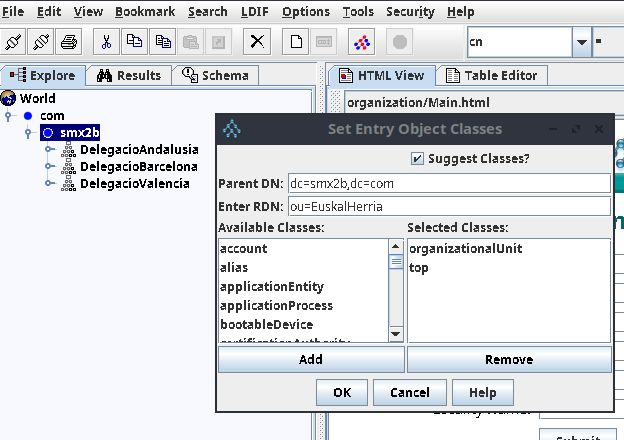
\includegraphics{png/jxplorerNovaOU.jpg}

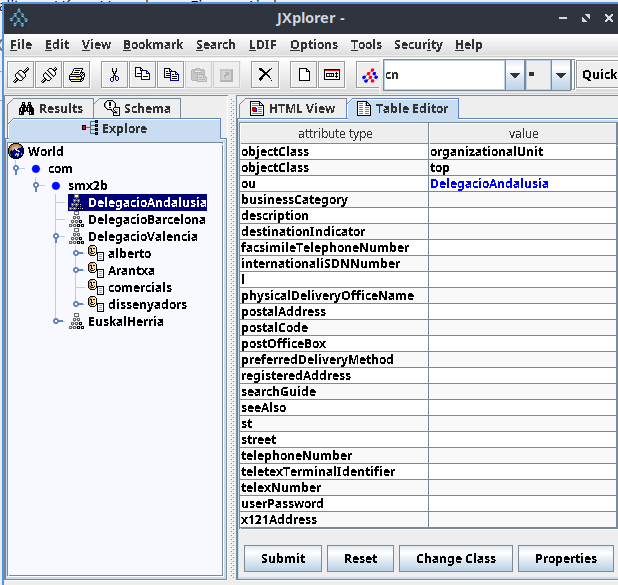
\includegraphics{png/atributsOU.png}

\begin{center}\rule{0.5\linewidth}{0.5pt}\end{center}

\subsubsection{Usuari del domini}\label{usuari-del-domini}

Un \textbf{usuari} ha de tenir atributs mínims per ser compatible amb
Linux, especialment per poder iniciar sessió i interactuar amb el
sistema.

\begin{itemize}
\tightlist
\item
  \textbf{Classes d'objecte necessàries:}

  \begin{itemize}
  \tightlist
  \item
    \texttt{top}
  \item
    \texttt{posixAccount} (indispensable per a compatibilitat amb Linux)
  \item
    \texttt{inetOrgPerson} (opcional, però útil per informació
    addicional de l'usuari)
  \end{itemize}
\item
  \textbf{Atributs obligatoris per Linux (\texttt{posixAccount}):}

  \begin{itemize}
  \tightlist
  \item
    \texttt{cn} (Common Name): Nom complet de l'usuari.
  \item
    \texttt{uid} (User ID): Identificador únic de l'usuari.
  \item
    \texttt{uidNumber}: Número d'usuari (ha de ser únic).
  \item
    \texttt{gidNumber}: Número de grup principal associat a l'usuari.
  \item
    \texttt{homeDirectory}: Ruta del directori personal de l'usuari.
  \item
    \texttt{loginShell}: Shell de connexió (exemple:
    \texttt{/bin/bash}).
  \end{itemize}
\end{itemize}

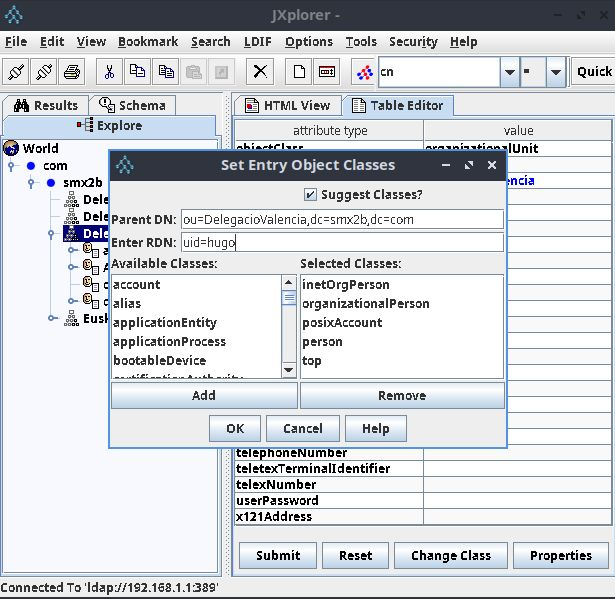
\includegraphics{png/jxplorerNouUsuari.jpg}
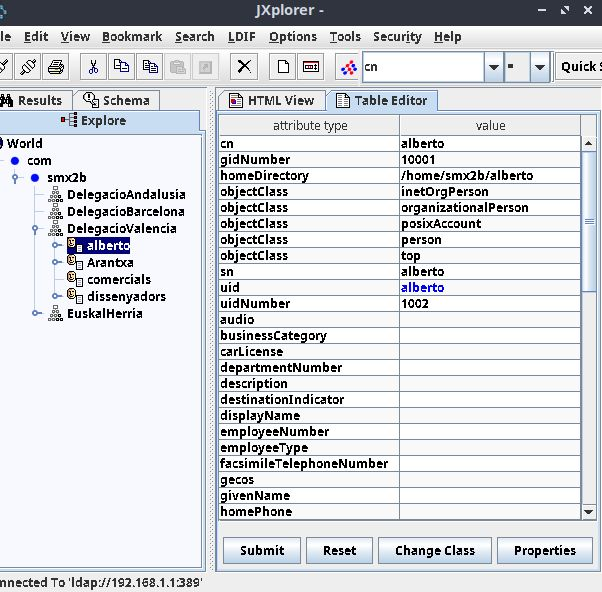
\includegraphics{png/atributsUsuari.jpg} ---

\subsubsection{Grup d'usuaris del
domini}\label{grup-dusuaris-del-domini}

Un \textbf{grup} ha de tenir atributs mínims per ser reconegut pel
sistema Linux i associar-se amb usuaris.

\begin{itemize}
\tightlist
\item
  \textbf{Classes d'objecte necessàries:}

  \begin{itemize}
  \tightlist
  \item
    \texttt{top}
  \item
    \texttt{posixGroup}
  \end{itemize}
\item
  \textbf{Atributs obligatoris per Linux (\texttt{posixGroup}):}

  \begin{itemize}
  \tightlist
  \item
    \texttt{cn} (Common Name): Nom del grup.
  \item
    \texttt{gidNumber}: Número de grup (ha de ser únic).
  \item
    \texttt{memberUid} (opcional, però recomanat): Identificadors dels
    usuaris que pertanyen al grup.
  \end{itemize}
\end{itemize}

Veiem què passa si falten propietats requerides:

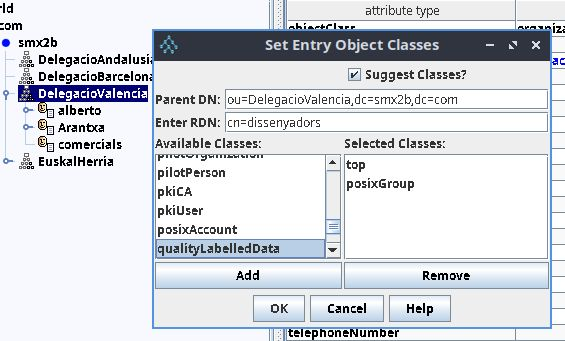
\includegraphics{png/jxplorerNouGrup1.jpg}

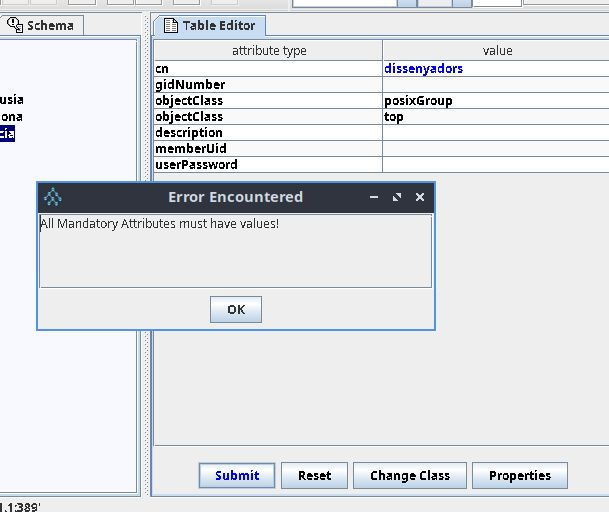
\includegraphics{png/jxplorerNouGrup2.jpg}

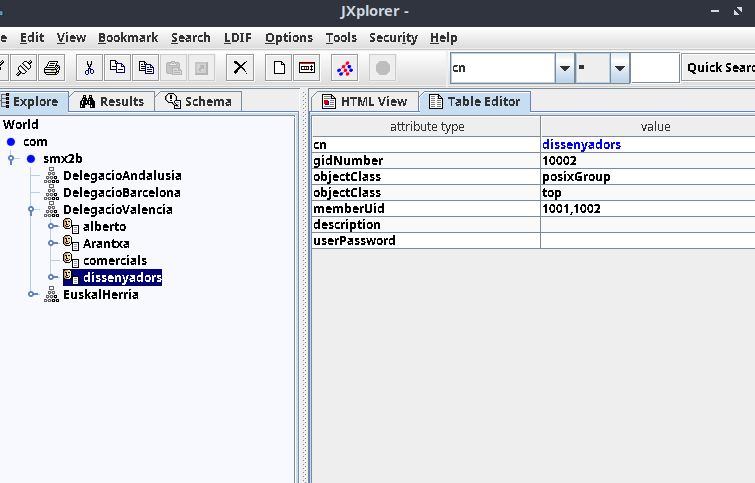
\includegraphics{png/jxplorerNouGrup3.jpg}

\begin{center}\rule{0.5\linewidth}{0.5pt}\end{center}

\begin{longtable}[]{@{}
  >{\raggedright\arraybackslash}p{(\columnwidth - 4\tabcolsep) * \real{0.2149}}
  >{\raggedright\arraybackslash}p{(\columnwidth - 4\tabcolsep) * \real{0.2645}}
  >{\raggedright\arraybackslash}p{(\columnwidth - 4\tabcolsep) * \real{0.5207}}@{}}
\toprule\noalign{}
\begin{minipage}[b]{\linewidth}\raggedright
\textbf{Tipus}
\end{minipage} & \begin{minipage}[b]{\linewidth}\raggedright
\textbf{Classes d'Objecte}
\end{minipage} & \begin{minipage}[b]{\linewidth}\raggedright
\textbf{Atributs Mínims Necessaris}
\end{minipage} \\
\midrule\noalign{}
\endhead
\bottomrule\noalign{}
\endlastfoot
\textbf{Unitat Organitzativa} & \texttt{top},
\texttt{organizationalUnit} & \texttt{ou} \\
\textbf{Usuari} & \texttt{top}, \texttt{posixAccount} & \texttt{cn},
\texttt{uid}, \texttt{uidNumber}, \texttt{gidNumber},
\texttt{homeDirectory}, \texttt{loginShell} \\
\textbf{Grup} & \texttt{top}, \texttt{posixGroup} & \texttt{cn},
\texttt{gidNumber}, (\texttt{memberUid} opcional però recomanat) \\
\end{longtable}

\begin{center}\rule{0.5\linewidth}{0.5pt}\end{center}

\subsection{6.3 Conceptes clau sobre objectes i classes a
LDAP}\label{conceptes-clau-sobre-objectes-i-classes-a-ldap}

\begin{enumerate}
\def\labelenumi{\arabic{enumi}.}
\tightlist
\item
  Les classes d'objecte defineixen els atributs i el comportament dels
  objectes:actua com una plantilla que especifica:

  \begin{itemize}
  \tightlist
  \item
    Quins atributs són obligatoris.
  \item
    Quins atributs són opcionals.
  \end{itemize}
\item
  Herència entre classes d'objecte

  \begin{itemize}
  \tightlist
  \item
    Exemple:
  \item
    La classe \texttt{inetOrgPerson} hereta d'altres classes com
    \texttt{organizationalPerson}, \texttt{person} i \texttt{top}.
  \end{itemize}
\item
  \textbf{Exemple d'herència en classes:} Si tens un usuari definit amb
  la classe \texttt{inetOrgPerson}, automàticament aquest objecte també
  hereta els atributs de les classes de les quals depèn. Veieu-ho
  gràficament:
\end{enumerate}

\emph{Diagrama d'herència}:

\begin{verbatim}
top
  person
       organizationalPerson
                          inetOrgPerson
\end{verbatim}

\subsection{6.3 Fitxers ldif}\label{fitxers-ldif}

Els vorem més avant però teniu ací un exemples amb les propietats
mínimes requerides.

\paragraph{Exemple d'una entrada d'OU:}\label{exemple-duna-entrada-dou}

\begin{Shaded}
\begin{Highlighting}[]
\NormalTok{dn: ou=usuaris,dc=exemple,dc=com}
\NormalTok{objectClass: top}
\NormalTok{objectClass: organizationalUnit}
\NormalTok{ou: usuaris}
\end{Highlighting}
\end{Shaded}

\paragraph{Exemple d'una entrada
d'usuari:}\label{exemple-duna-entrada-dusuari}

\begin{Shaded}
\begin{Highlighting}[]
\NormalTok{dn: uid=jordi,ou=usuaris,dc=exemple,dc=com}
\NormalTok{objectClass: top}
\NormalTok{objectClass: posixAccount}
\NormalTok{objectClass: inetOrgPerson}
\NormalTok{cn: Jordi Gómez}
\NormalTok{sn: Gómez}
\NormalTok{uid: jordi}
\NormalTok{uidNumber: 1001}
\NormalTok{gidNumber: 1001}
\NormalTok{homeDirectory: /home/jordi}
\NormalTok{loginShell: /bin/bash}
\end{Highlighting}
\end{Shaded}

\subsubsection{Exemple pràctic: Usuari amb múltiples
classes}\label{exemple-pruxe0ctic-usuari-amb-muxfaltiples-classes}

Un usuari que és compatible amb Linux i també conté informació personal
pot definir-se així:

\begin{Shaded}
\begin{Highlighting}[]
\NormalTok{dn: uid=jordi,ou=usuaris,dc=exemple,dc=com}
\NormalTok{objectClass: top}
\NormalTok{objectClass: person}
\NormalTok{objectClass: organizationalPerson}
\NormalTok{objectClass: inetOrgPerson}
\NormalTok{objectClass: posixAccount}
\NormalTok{cn: Jordi Gómez}
\NormalTok{sn: Gómez}
\NormalTok{uid: jordi}
\NormalTok{uidNumber: 1001}
\NormalTok{gidNumber: 1001}
\NormalTok{homeDirectory: /home/jordi}
\NormalTok{loginShell: /bin/bash}
\NormalTok{mail: jordi@example.com}
\NormalTok{telephoneNumber: +34 600 123 456}
\end{Highlighting}
\end{Shaded}


\end{document}
